%\documentclass[12pt]{report}
%\documentclass[12pt]{extreport}
\documentclass[17pt]{extarticle}
\usepackage{graphicx}
\usepackage{setspace}
\usepackage{amsmath,amssymb}
\usepackage{IEEEtrantools}
\usepackage{cancel}

\usepackage{geometry}
 \geometry{
 a4paper,
 total={170mm,264mm},
 left=20mm,
 top=10mm,
 }

\begin{document}


\section{Esercizio}

Due punti materiali, sono vincolati a muoversi su di una guida circolare di raggio $r = 15 cm$. Ad un certo istante i due punti occupano la stessa posizione e si muovono in versi opposti con velocit\'a di modulo costante, pari a $v_1 = 3m/s$ e $v_2 = 6m/s$. Determinare dopo quanto tempo si incontrano di nuovo e l'arco di traiettoria percorsa da ciascuno dei due punti.\\



\begin{minipage}{0.35\textwidth}
{\bf Dati}
\begin{itemize}
		\item $r = 15$ $cm$\\
		\item $V_1 = 3$ $m/s$\\
		\item $V_2 = 6$ $m/s$\\
	\end{itemize}
\end{minipage}%
\hfill
\begin{minipage}{0.65\textwidth}
	\begin{tabular}{|p{\textwidth}}		
		\centering
    	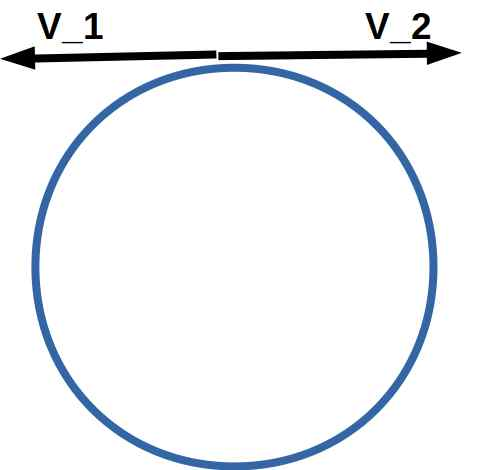
\includegraphics[width=2.0in]{Clipboard01.jpg}
    	\label{fig:sample_figure}		
	\end{tabular}
	
\end{minipage}%

\vspace{10mm}

Secondo definizione, la velocit\'a angolare \'e
{ \Large \begin{IEEEeqnarray}{lCr}
	\omega = \frac{\Delta \alpha}{\Delta t} = \frac{v}{r}
\end{IEEEeqnarray} }

Usiamo i pedici 1 e 2 per identificare le grandezze di, rispettivamente, il primo e il secondo punto materiale


{ \Large \begin{IEEEeqnarray}{lCr}
 {\setstretch{2.25}%Distance between two following lines
\left\{ \begin{array}{ccc}
\omega_1 & = & \frac{V_1}{r} = \frac{\Delta\alpha_1}{\Delta t} \\ 
\omega_2 & = & \frac{V_2}{r} = \frac{2\pi - \Delta\alpha_1}{\Delta t}
\end{array}
\right. } \label{eq:sistema}
\end{IEEEeqnarray} }


Esplicitando $\Delta t$ nella prima delle equazioni \ref{eq:sistema} 
\begin{equation}
	\Delta t = \frac{\Delta \alpha_1 r}{V_1}
\end{equation}

E sostituendo nella seconda, si ha

\begin{eqnarray}
	\frac{V_2}{r} & = & \frac{2\pi - \Delta\alpha_1}{\Delta\alpha_1 r/V_1} \label{eq:dopo}
\end{eqnarray}

e quindi

\begin{eqnarray}
	\nonumber & \frac{\Delta \alpha_1\cancel{r} }{V_1}\cdot\frac{V_2}{ \cancel{r} } = 2\pi - \Delta\alpha_1 \\ 
	\nonumber & \Delta \alpha_1\cdot\frac{V_2}{V_1} = 2\pi - \Delta\alpha_1\\ 
	\nonumber & \Delta\alpha_1\frac{V_2}{V_1} + \Delta\alpha_1 = 2\pi\\ 
	\nonumber & \Delta\alpha_1 \left(\frac{V_2}{V_1} + 1 \right) = 2\pi 
\end{eqnarray}

E quindi l'angolo descritto dal primo punto materiale, quello descritto dal secondo e il tempo richiesto sono
\begin{eqnarray}
	\Delta\alpha_1 = \frac{2\pi V_2}{V_1 + V_2}\qquad \Delta\alpha_2 = 2\pi - \alpha_1 \qquad \Delta t = \frac{\Delta\alpha_1r}{V_2}
\end{eqnarray}

Mettendo i numeri
\begin{eqnarray}
	& & \Delta\alpha_1 = \frac{2\pi \cdot 3m/s}{3m/s + 6m/s} = 0.70 rad\\
	& & \Delta\alpha_2 = 5.58 rad \\
	& & \Delta t = \frac{0.70rad \cdot 0.15}{6m/s} = 0.017 s
\end{eqnarray}

\section{Esercizio}


Un corpo di massa $m_1$ pu\'o scorrere senza attrito su di una superficie orizzontale. Due fili inestensibili e di massa trascurabile lo collegano, tramite due carrucole fisse e lisce, con due corpi di massa $m_2$ e $m_3$ (vedi figura in allegato). Se $m_2$ diverso da $m_3$, il sistema si mette in moto. Calcolare il modulo della accelerazione della massa $m_1$, se $m_1 = m_2$ e $m_3 = 2m_2$.

\vspace{1.5cm}


	\begin{tabular}{p{\textwidth}}		
		\centering
    	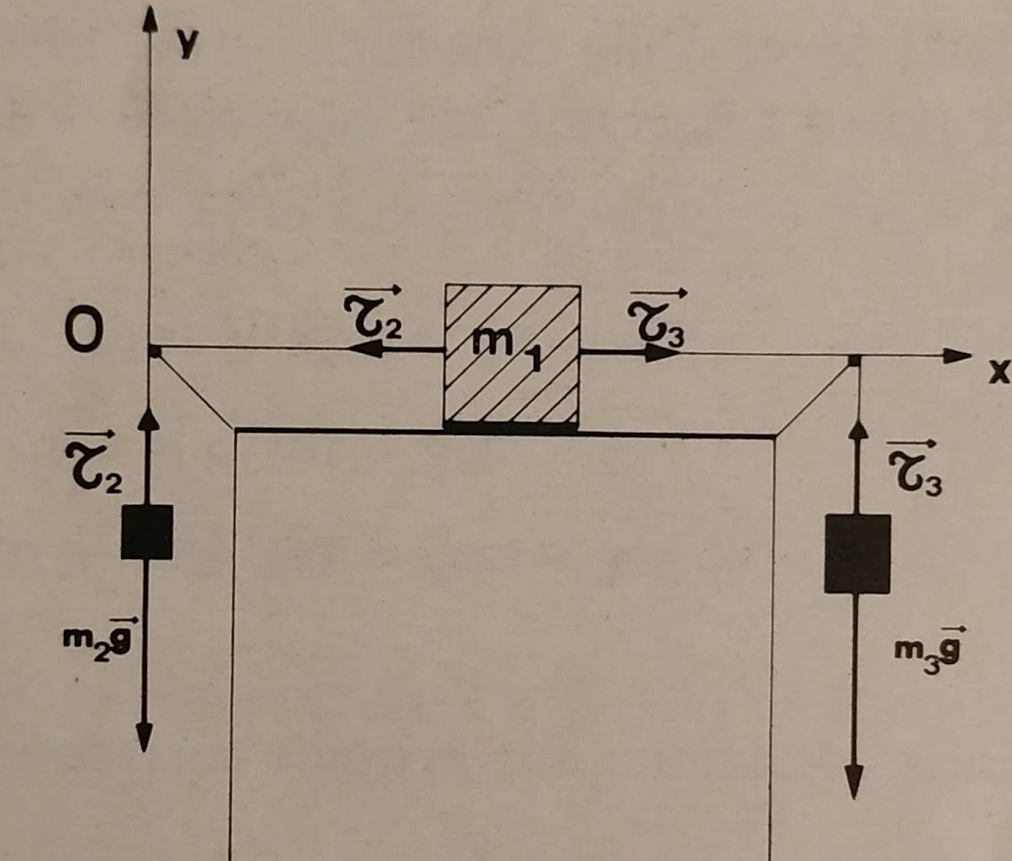
\includegraphics[width=2.5in]{EsercizioCarrucole.png}
    	\label{fig:sample_figure}		
	\end{tabular}


%{ \Large 
\begin{IEEEeqnarray}{lCr}
 {\setstretch{2.25}%Distance between two following lines
\left\{ \begin{array}{ccc}
m_3a & = & m_3g - \tau_3 \\ 
m_1a & = & \tau_3 - \tau_2\\
m_2a & = & -m_2g + \tau_2
\end{array}
\right. } \label{eq:sistema}
\end{IEEEeqnarray} 
%}

Secondo l'esercizio $m_1 = m_2$ e $m_3 = 2m_2$. Chiamo $m = m_1$ e quindi posso scrivere

%{ \Large 
\begin{IEEEeqnarray}{lCr}
 {\setstretch{2.25}%Distance between two following lines
\left\{ \begin{array}{ccc}
2ma & = & 2mg - \tau_3 \\ 
ma & = & \tau_3 - \tau_2\\
ma & = & -mg + \tau_2
\end{array}
\right. } \label{eq:sistema}
\end{IEEEeqnarray} %}

L'ultima equazione diventa 

\begin{equation}
	\tau_2 = ma + mg = m(a +g)
\end{equation}

e quindi

%{ \Large 
\begin{IEEEeqnarray}{lCr}
 {\setstretch{2.25}%Distance between two following lines
\left\{ \begin{array}{ccc}
2ma & = & 2mg - \tau_3 \\ 
ma & = & \tau_3 - \tau_2\\
\tau_2 & = & ma + mg = m(a +g)
\end{array}
\right. } \label{eq:sistema}
\end{IEEEeqnarray} %}

Sostituendo l'espressione di $\tau_2$ nell'ultima equazione, la penultima equazione la si pu\'o scrivere
\begin{eqnarray}
	\tau_3 = ma + m(a+g) = m(2a+g)
\end{eqnarray}

Che, sostituita nella prima, si ha
\begin{eqnarray}
	\nonumber & 2\cancel{m}g -\cancel{m}(2a+g)=2\cancel{m}a\\
	& 2g -2a - g = 2a
\end{eqnarray}

Ossia
\begin{equation}
	a = g/4 = 9.81m/s^2/4 = 2.45m/s^2
\end{equation}

\section{Pag 279 n 62}

L'equazione del momento della forza \'e 

\begin{eqnarray}
	M = I\dot{\omega}
\end{eqnarray}

Il momento d'inerzia $I$ di una asta omogenea di lunghezza $l$, rispetto ad un asse passante per il centro di massa \'e 

\begin{eqnarray}
	I_{cm} = \frac{1}{12}ml^2
\end{eqnarray}

L'asta \'e vincolata a muoversi attorno ad una sua estremit\'a , distante $l/2$ dal centro di massa, il momento d'inerzia \'e

\begin{eqnarray}
	I = I_{cm} + mr^2
\end{eqnarray}

ove $r$ \'e la distanza dell'asse di rotazione rispetto al centro di massa e vale la met\'a della lunghezza dell'asta stessa $l/2$. Quindi il momento d'inerzia vale

\begin{eqnarray}
	I = \frac{1}{12}ml^2 + m\left(\frac{l}{2}\right)^2 = \frac{1}{3}ml^2
\end{eqnarray}


La forza che agisce sul corpo \'e la forza peso che, ancora una volta, si applica al centro di massa. Nell'istante iniziale forza e braccio sono tra loro perpendicolari e il momento $M$ \'e

\begin{eqnarray}\label{eq:momento}
	M = mgl/2
\end{eqnarray}

Quindi, mettendo insieme i risultati ottenuti si ha
\begin{eqnarray}\nonumber
	\frac{1}{3}\cancel{m}L^2\dot{\omega} = \cancel{m}g\frac{L}{2}\\
	\frac{1}{3}L\dot{\omega} = g\frac{1}{2}
\end{eqnarray}

Da cui si deduce che 
\begin{equation}
	\dot{\omega} = \frac{3g}{2L}
\end{equation}

Questo \'e l'accelerazione dell'asta quando si trova disposta orizzontalemente, nell'istante in cui viene lasciata ruotare attorno al perno. L'accelerazione nell'istante in cui forma un angolo di 30 gradi con l'orizzontale va fatta tenendo conto che il momento \'e un prodotto vettoriale tra forza e braccio e, in quanto tale, il suo modulo \'e $Fb\sin{\alpha}$, ove $\alpha$ \'e l'angolo che i due vettori, forza e braccio formano tra loro. Nel caso specifico $\pi/3$. L'accelerazione angolare, quindi, \'e
\begin{eqnarray}
	\dot{\omega} = \frac{3g\sin{\pi/3} }{2L} = \frac{3\cdot 9.8 \cancel{m}/s^2}{2\cdot 0.5 \cancel{m}}\frac{\sqrt{3}}{2} = 25.5rad/s^2
\end{eqnarray}

\end{document}